\documentclass{article}
\usepackage[preprint]{neurips_2025}
\usepackage[utf8]{inputenc}
\usepackage[T1]{fontenc}
\usepackage{hyperref}
\usepackage{url}
\usepackage{booktabs}
\usepackage{amsfonts,amsmath}
\usepackage{nicefrac}
\usepackage{microtype}
\usepackage{xcolor}
\usepackage{graphicx}

\newcommand{\ros}{R^2_{\mathrm{OS}}}

\title{Can Past Anomaly Returns Time the Anomalies?\\Regularized Out-of-Sample Forecasts of Long-Short Portfolio Returns}

\author{%
  Saranya Anantapantula \And David Cheng \And Peter Ilyin\\
  ESE 4020, University of Pennsylvania
}

\begin{document}
\maketitle

\begin{abstract}
Do the past returns of published stock-market anomaly portfolios forecast next month's return of each portfolio better than its historical mean, out of sample? We use the Open Source Asset Pricing long-short returns (Chen \& Zimmermann), forecast each portfolio from 12 monthly lags of all portfolios with ridge (the course baseline), lasso and elastic net, and tune every penalty by blocked 5-fold cross-validation inside an expanding training window. On a 1990--2009 validation window, with 12-month block-bootstrap intervals, no method beats the historical mean: out-of-sample $R^2$ ranges from \textbf{+0.03\% to +1.4\%} with intervals that always contain zero, and forecast-sign timing Sharpe ratios are within the bootstrap interval of buy-and-hold; the closest call is lasso on all 152 signals ($+0.30$ Sharpe, interval $[-0.002, +0.56]$). The small gains come from a handful of crisis months; ridge's timing edge disappears at any trading cost and the sparse models' at about 0.3--0.6\% one-way. The 2010--2024 final period is untouched and will be evaluated once.
\end{abstract}

%======================================================================
\section{Introduction}
\textbf{Question.} Academic finance has documented over two hundred cross-sectional ``anomalies'': stock characteristics whose top-minus-bottom (long-short) portfolio earns a positive average return. Holding such a portfolio all the time is the default. \emph{Factor timing} asks whether one can do better by changing the exposure month to month. We ask a narrow, testable version: \emph{does a regularized linear model of the past returns of all anomaly portfolios forecast next month's return of each portfolio better than that portfolio's historical mean, out of sample?}

\textbf{Why it matters.} Two literatures disagree. Goyal and Welch~\cite{goyal2008} show that most return predictors fail to beat the historical mean out of sample, while Haddad, Kozak and Santosh~\cite{hks2020} argue that anomaly returns are predictable enough for timing to be valuable. Anomaly returns also decay after publication~\cite{mclean2016}, so a test that uses signals before anyone knew them overstates what an investor could have done. A clean answer needs strictly chronological evaluation, honest tuning and error bars that respect serial dependence in monthly returns.

\textbf{What we compare.} The historical mean is the benchmark. Against it we compare (i) OLS on each portfolio's own last-month and 12-month mean return, (ii) ridge regression on the lags of all portfolios, the course baseline, and (iii) lasso and elastic net on the same inputs and folds. We run every method on three universes: the 5 signals of our baseline, all 152 signals observed throughout 1972--2009, and a point-in-time universe that only uses signals already published.

%======================================================================
\section{Data}
\textbf{Source.} Open Source Asset Pricing (OSAP), data release 2025.10, file \texttt{Portfolios/Full Sets OP/PredictorLSretWide.parquet}, and the signal documentation \texttt{SignalDoc.csv}; \url{https://huggingface.co/datasets/OpenSourceAP/CrossSection} (branch \texttt{2025.10}). OSAP rebuilds each published predictor from CRSP and Compustat and forms the long-short portfolio as in the original paper (quantile, weighting and rebalancing as published)~\cite{chen2022}. The public files contain portfolio returns but no firm-level returns, which is why our target is a portfolio return.

\textbf{Size and shape.} The wide file is 1{,}188 months (Jan 1926--Dec 2024) $\times$ 212 predictors of monthly long-short returns in percent, with missing values before each signal starts. \texttt{SignalDoc.csv} gives the publication year of each of the 331 documented signals. The 5-signal baseline files (AnnouncementReturn, BetaFP, Mom12m, MomSeasonShort, STreversal) match the wide file to $10^{-16}$.

\textbf{Universes.} \emph{5 signals}: Nov 1971--Dec 2009 (Sep--Oct 1971 dropped because one leg held fewer than 100 stocks), 12 lags $\times$ 5 = 60 inputs. \emph{152 signals}: every signal with no missing month from Jan 1972 to Dec 2009, giving 12 $\times$ 152 = 1{,}824 inputs. This set is chosen with pre-2010 data only, so the final period plays no role in it. \emph{Published}: at each scored year $Y$, only signals whose publication year is before $Y$ serve as inputs and targets. This universe grows from 12 portfolios (144 inputs) in 1990 to 119 (1{,}428 inputs) in 2009.

\textbf{Split.} Strict time order; nothing is shuffled. \emph{Final evaluation}: Jan 2010--Dec 2024 (180 months). Our code drops these rows when it loads the data, so no model, penalty or design choice has seen them. \emph{Validation}: Jan 1990--Dec 2009 (240 months). It is scored by 20 annual refits, each trained on all months up to 12 months before the scored year. \emph{Training}: the expanding window from 1972 (192 months for the 1990 refit, 420 for 2009).

%======================================================================
\section{Method}
Let $r_{j,t}$ be the return of portfolio $j$ in month $t$ and $x_t=(r_{k,t-\ell})_{k,\ell=1..12}$ the lags of all $N$ portfolios, standardized with training-window means and standard deviations. Every model below forecasts $\hat r_{j,t}$ with a separate regression per portfolio. Within a model, all portfolios share one penalty.
\begin{itemize}
\item \textbf{Historical mean (benchmark).} $\hat r_{j,t}=$ mean of $r_j$ over the training window.
\item \textbf{OLS on established signals.} $r_{j,t}$ on $r_{j,t-1}$ and the 12-month mean $\bar r_{j,t-12:t-1}$ (5-signal universe only).
\item \textbf{Ridge (course baseline).} $\min_b \|y-Xb\|^2+\alpha\|b\|_2^2$; grid $\alpha\in\{10^0,\dots,10^8\}$, 33 log-spaced values. The baseline checkpoint used $10^0$--$10^6$; we widened it for 1{,}824 inputs.
\item \textbf{Lasso.} $\min_b \tfrac{1}{2n}\|y-Xb\|^2+\alpha\|b\|_1$; grid $\alpha\in\{10^{-2},\dots,10^{1}\}$, 13 log-spaced values, in units of percent return. At the top of the grid every coefficient is zero and lasso \emph{equals} the historical mean, so the model can fall back to the benchmark.
\item \textbf{Elastic net.} The same with penalty $\alpha(\rho\|b\|_1+\tfrac{1-\rho}{2}\|b\|_2^2)$, $\rho=0.5$ fixed in this draft, same grid.
\end{itemize}
\textbf{Tuning.} In every annual refit, the penalty is chosen by \emph{blocked 5-fold cross-validation inside that refit's training window}: five contiguous folds, with 12 months purged on each side of the held-out fold so that overlapping lag windows cannot leak, and scaling refit on the training folds. The criterion is squared error pooled over portfolios. The final model is refit on the full training window with the chosen penalty. None of the chosen ridge, lasso or elastic-net penalties lies on a grid edge in any refit.

%======================================================================
\section{Experimental setup}
\textbf{Metrics.} (1) Pooled out-of-sample $R^2$ against the historical mean, $\ros=1-\sum_{j,t}(r_{j,t}-\hat r_{j,t})^2/\sum_{j,t}(r_{j,t}-\bar r_{j,t})^2$ over all validation forecasts; $\ros>0$ means the model beats the benchmark. (2) A \emph{timing Sharpe ratio}: each month, hold every portfolio long or short according to the sign of its forecast, equal-weighted, and annualize mean/s.d. Because historical means are almost always positive, the benchmark strategy is roughly buy-and-hold. (3) \emph{Turnover} $\sum_j|w_{j,t}-w_{j,t-1}|$ and the net return $s_t-2c\cdot\text{turnover}_t$ for a one-way cost $c$ per leg, plus the \emph{break-even cost} at which a model's net Sharpe falls to the benchmark's.

\textbf{Validation.} All numbers in this draft come from the 1990--2009 validation window, which is out of sample for every refit. The 2010--2024 period will be evaluated once, after the specification is frozen.

\textbf{Error bars.} Monthly returns are serially dependent and cross-correlated, so we resample whole months (all portfolios together) with a circular block bootstrap: 12-month blocks, 2{,}000 draws, 95\% percentile intervals, seed 4020. Each draw recomputes the metric from the resampled forecast--outcome pairs. Sharpe \emph{differences} are bootstrapped jointly, so they are paired. Following the course convention, \emph{a gain inside its interval is a tie}.

%======================================================================
\section{Preliminary results}
\begin{table}[t]
\caption{Validation results, Jan 1990--Dec 2009 (240 months). $\ros$ is against the historical mean. Brackets are 95\% circular block-bootstrap intervals (12-month blocks, 2{,}000 draws). Sharpe: annualized, forecast-sign timing, equal-weighted. Turnover: mean monthly $\sum_j|\Delta w_j|$. Break-even: one-way cost per leg (\%) at which net Sharpe equals the historical mean's; 0 means the model is already behind before costs. Forecasts: 1{,}200 (5 signals), 36{,}480 (152 signals), 10{,}656 (published only). $^\dagger$OLS from the baseline-checkpoint run.}
\label{tab:main}
\centering
\footnotesize
\setlength{\tabcolsep}{4pt}
\begin{tabular}{llcccc}
\toprule
Universe & Model & $\ros$ (\%) & Sharpe & Sharpe $-$ HM & Break-even \\
\midrule
5 signals & Hist.\ mean & 0 & 0.99 & --- & --- \\
& OLS$^\dagger$ & $-2.05$ [$-3.06$, $-0.73$] & 0.88 & --- & --- \\
 & Ridge & $+0.06$ [$-5.93$, $+4.38$] & 0.96 & $-0.03$ [$-0.51$, $+0.37$] & 0 \\
 & Lasso & $+0.26$ [$-5.33$, $+4.07$] & 1.18 & $+0.19$ [$-0.19$, $+0.49$] & 0.63 \\
 & Elastic net & $+0.78$ [$-5.58$, $+5.06$] & 1.00 & $+0.01$ [$-0.37$, $+0.30$] & 0.02 \\
\midrule
152 signals & Hist.\ mean & 0 & 1.81 & --- & --- \\
& Ridge & $+0.03$ [$-2.67$, $+3.45$] & 1.78 & $-0.02$ [$-0.55$, $+0.38$] & 0 \\
 & Lasso & $+0.24$ [$-2.97$, $+2.98$] & 2.11 & $+0.30$ [$-0.002$, $+0.56$] & 0.39 \\
 & Elastic net & $+0.98$ [$-2.04$, $+4.10$] & 2.07 & $+0.26$ [$-0.02$, $+0.51$] & 0.27 \\
\midrule
Published only & Hist.\ mean & 0 & 1.27 & --- & --- \\
& Ridge & $+0.96$ [$-2.05$, $+5.52$] & 1.30 & $+0.03$ [$-0.47$, $+0.59$] & 0.02 \\
 & Lasso & $+1.39$ [$-4.61$, $+6.56$] & 1.50 & $+0.23$ [$-0.20$, $+0.81$] & 0.27 \\
\bottomrule
\end{tabular}
\end{table}

\begin{figure}[t]
\centering
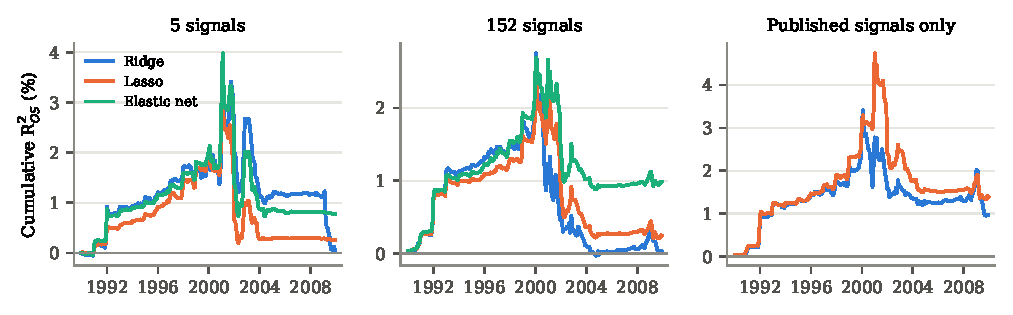
\includegraphics[width=\linewidth]{figs/cum_r2.pdf}
\caption{Cumulative out-of-sample $R^2$ against the historical mean through the validation window, scaled so the last value equals the full-window $\ros$ in Table~\ref{tab:main}. A rising line means the model is beating the historical mean that month. In every universe, most of the gain is made around 2000--2001 and given back in 2001--2003 and the 2009 momentum crash.}
\label{fig:cum}
\end{figure}

\begin{figure}[t]
\centering
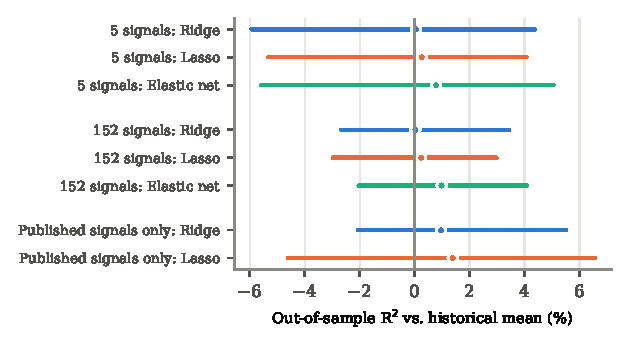
\includegraphics[width=0.62\linewidth]{figs/r2_ci.pdf}
\caption{$\ros$ (dots) with 95\% block-bootstrap intervals (bars) for each model and universe. Every interval contains zero: no method beats the historical mean.}
\label{fig:ci}
\end{figure}

\textbf{The baseline is a tie.} With 5 signals, ridge's $\ros$ is $+0.06\%$ with an interval of roughly $\pm5$ percentage points. OLS on own-portfolio momentum is significantly \emph{worse} than the historical mean. Lasso and elastic net are also ties (Table~\ref{tab:main}, Figure~\ref{fig:ci}). Moving to all 152 signals (1{,}824 inputs) narrows the $\ros$ intervals but does not move the point estimates away from zero. The one result near the edge is timing: lasso and elastic net beat buy-and-hold by $+0.30$ and $+0.26$ Sharpe, with lower interval bounds of $-0.002$ and $-0.02$. That is still a tie, and it is the best of nine model--universe comparisons, so we treat it as a hypothesis to test on the final period, not a finding. The contrast with $\ros\approx0$ suggests the sparse models get the \emph{sign} of next month's return right slightly more often without reducing squared error.

\textbf{Gains are episodic.} Figure~\ref{fig:cum} shows that the cumulative advantage builds slowly through the 1990s, jumps in 2000--2001, and is mostly given back in 2001--2003 and in 2009. A handful of crisis months decide the sign of $\ros$, which is why the intervals are wide.

\textbf{Sparsity.} Lasso keeps very few inputs: 1--5 of 60 with 5 signals, 2--10 of 1{,}824 with 152 signals. After 2004 it keeps almost none, so its forecast collapses to the historical mean. Ridge forecasts move about 12 times as much as the historical mean's (monthly s.d.\ 1.61\% vs.\ 0.13\% with 5 signals), so ridge is noisier, not more informative.

\textbf{Point-in-time.} Restricting to published signals \emph{raises} every Sharpe ratio, because the targets change: published anomalies earned more over 1990--2009 than the not-yet-published ones. The model-minus-benchmark differences remain ties.

\textbf{Costs.} Sign-timing turns portfolios over. Ridge's edge vanishes at a one-way cost of about 0.02\%. Lasso's edge survives to 0.27--0.63\%, but that edge was never statistically distinguishable from zero.

%======================================================================
\section{Remaining sections and experiments before Analysis Complete (30 November)}
\textbf{Outline of the remaining paper.} \S6 Analysis: where the gains come from (crisis months, per-portfolio $\ros$, which lags lasso selects); \S7 Final evaluation on 2010--2024, run once with the frozen specification; \S8 Limitations; \S9 Conclusion.

\textbf{Experiments still to run} (all on the validation window; the final period stays untouched until the specification is frozen):
\begin{enumerate}
\item \textbf{Tune the elastic-net mix} $\rho\in\{0.1,0.5,0.9\}$ jointly with $\alpha$ by the same CV (fixed at 0.5 in this draft for compute).
\item \textbf{Elastic net on the point-in-time universe}, and a variant that filters only the targets (not the inputs) by publication date.
\item \textbf{Principal-component timing}~\cite{hks2020}: forecast the first few principal components of anomaly returns (estimated in each training window) and map back to portfolios. This is the main alternative to regressing on raw lags.
\item \textbf{Robustness}: 1, 3 and 6 lags instead of 12; 6- and 24-month bootstrap blocks; per-portfolio penalties instead of a shared one; $\ros$ with and without 2000--2003 and 2009; per-portfolio $\ros$ with intervals.
\item \textbf{Costs}: report net Sharpe at 0.10/0.25/0.50\% with intervals. The OSAP portfolios' own rebalancing costs are not in the data, but both the timed and buy-and-hold strategies pay them.
\item \textbf{Freeze and test}: choose one specification on validation only, then evaluate 2010--2024 once with the same metrics and intervals.
\end{enumerate}

\textbf{Known limitations to address.} The wide file has no stock counts per leg, so the thin-leg filter applies only to the 5-signal run. Publication dates are years, not months. In the point-in-time universe, models still train on a signal's pre-publication history, which is the in-sample period of the original paper, so those returns may be inflated~\cite{mclean2016}.

\begin{thebibliography}{9}
\small
\bibitem{chen2022} A.~Y.~Chen and T.~Zimmermann. Open source cross-sectional asset pricing. \emph{Critical Finance Review}, 11(2):207--264, 2022.
\bibitem{goyal2008} A.~Goyal and I.~Welch. A comprehensive look at the empirical performance of equity premium prediction. \emph{Review of Financial Studies}, 21(4):1455--1508, 2008.
\bibitem{hks2020} V.~Haddad, S.~Kozak, and S.~Santosh. Factor timing. \emph{Review of Financial Studies}, 33(5):1980--2018, 2020.
\bibitem{mclean2016} R.~D.~McLean and J.~Pontiff. Does academic research destroy stock return predictability? \emph{Journal of Finance}, 71(1):5--32, 2016.
\end{thebibliography}

\end{document}
